\section{Computing Fourier Series and Transforms}

\subsection{Introduction}
\begin{frame}{Introduction}
    \begin{itemize}[<+->]
      \item Using the Fourier techniques we can obtain the frequency-domain representation of signals.
      \item We use Fourier series for periodic signals, and Fourier transform for aperiodic signals.
      \item Each of these have continuous-time and discrete-time versions:
        \begin{enumerate}
            \item Continuous-time Fourier series
            \item Continuous-time Fourier transform
            \item Discrete-time Fourier series
            \item Discrete-time Fourier transform
        \end{enumerate}
      \item In this part of the course, we will concentrate on how to actually compute these. Later, after we study liner, time-invariant (LTI) systems, we will study the conceptual aspects of Fourier techniques.
    \end{itemize}
\end{frame}

\begin{frame}
    \begin{columns}[t]
        \begin{column}{0.4\textwidth}
            \begin{figure}
              \centering
              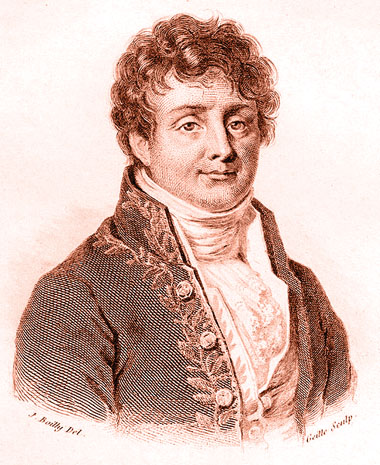
\includegraphics[width=0.4\textwidth]{figures/fourier.jpg}
              \caption{Jean-Baptiste Joseph Fourier, 1768--1830, French mathematician who discovered Fourier series and transform}\label{fi:secb_fourier}
            \end{figure}
        \end{column}
        \begin{column}{0.6\textwidth}
            \begin{itemize}[<+->]
              \item Every signal has a frequency distribution or a \alert{spectrum}.
              \item Periodic signals have a line spectra, called the Fourier series.
              \item The French mathematician, Jean-Baptiste Joseph Fourier, discovered this representation.
              \item Fourier series provides a way  to represent a periodic signal as a sum of complex sinusoids.
              \item These sinusoids will be at frequencies that are integer multiples of the fundamental frequency $\omega_0$.
              \item $\omega_0 = \frac{2\pi}{T}$, where $T$: fundamental period of the waveform.
            \end{itemize}
        \end{column}
    \end{columns}
\end{frame}

\subsection{Fourier Series}

\begin{frame}{Continuous-Time Fourier Series}
    \begin{equation}\label{eq:secb_fourierseries}
        \begin{aligned}
            x(t) &= \sum_{k=-\infty}^{+\infty}a_k e^{jk\omega_0 t}\\
            a_k &= \frac{1}{T} \int_{T}x(t)e^{-jk\omega_0 t}dt\\
            \omega_0 &= \frac{2\pi}{T}
        \end{aligned}
    \end{equation}
    The set of coefficients $\left\{a_k\right\}$ is called the \alert{Fourier series coefficients} of the \alert{spectral coefficients} of $x(t)$.
    The coefficient $a_0$ is the dc or constant component of $x(t)$, given by Equation \ref{eq:secb_fourierseries} with $k=0$:
    \begin{equation}\label{eq:secb_a0}
        a_0 = \frac{1}{T} \int_{T}x(t)dt,
    \end{equation}
    which is simply the average of $x(t)$ over one period.
\end{frame}

\begin{frame}
    \begin{example}
        Let
        \begin{equation*}
            x(t) = 1 + \sin \omega_0t + 2\cos\omega_0t+ \cos\left(2\omega_0t+ \frac{\pi}{4}\right),
        \end{equation*}
        which has the fundamental frequency $\omega_0$.
        \begin{enumerate}
            \item Use Euler's formula to express $x(t)$ as a liner combination of complex exponentials.
            \item Find the Fourier series coefficients, $a_k$.
            \item Plot the magnitude and phase of $a_k$.
        \end{enumerate}

    \end{example}
\end{frame}

\begin{frame}<beamer>[plain,t]
        \begin{equation*}
            x(t) = 1 + \sin \omega_0t + 2\cos\omega_0t+ \cos\left(2\omega_0t+ \frac{\pi}{4}\right),
        \end{equation*}

        Using Euler's formula
        \begin{equation*}
            x(t) = 1 + \frac{1}{2j}\left[e^{j\omega_0 t} - e^{-j\omega_0 t}\right] + \left[e^{j\omega_0 t} + e^{-j\omega_0 t}\right] + \frac{1}{2}\left[e^{j(2\omega_0 t + \pi/4)} + e^{-j(2\omega_0 t + \pi/4)}\right]
        \end{equation*}
        Collecting terms,
        \begin{equation*}
            x(t) = 1 + \left(1 + \frac{1}{2j}\right)e^{j\omega_0 t} +  \left(1 - \frac{1}{2j}\right)e^{-j\omega_0 t} + \left(\frac{1}{2} e^{j\pi/4}\right)e^{j2\omega_0 t} + \left(\frac{1}{2} e^{-j\pi/4}\right)e^{-j2\omega_0 t}
        \end{equation*}
        \begin{columns}
            \begin{column}{0.5\textwidth}
                The Fourier coefficients are
                \begin{equation*}
                    \begin{split}
                        a_0 &= 1,\\
                        a_1 &= \left(1 + \frac{1}{2j}\right) = \left(1 - \frac{j}{2}\right),
                    \end{split}
                \end{equation*}
            \end{column}
            \begin{column}{0.5\textwidth}
                \begin{equation*}
                    \begin{split}
                        a_{-1} &= \left(1 + \frac{1}{2j}\right) = \left(1 + \frac{j}{2}\right),\\
                        a_2 &= \frac{1}{2}e^{j\pi/4} = \frac{\sqrt{2}}{4}(1+j),\\
                        a_{-2} &= \frac{1}{2}e^{-j\pi/4} = \frac{\sqrt{2}}{4}(1-j),\\
                        a_k &= 0, |k|>2.
                    \end{split}
                \end{equation*}
            \end{column}
        \end{columns}

\end{frame}

\begin{frame}<beamer>[plain,t]
    \begin{figure}
      \centering
      \begin{tikzpicture}
	\def\w{{-3, -2, -1,0,1, 2, 3}}
	\def\akmag{{0, 0.5, 1.1180,  1, 1.1180, 0.5, 0}}
	\def\akarg{{0, -0.7854, 0.4636, 0, -0.4636, 0.7854, 0}}

	\begin{scope}	
		\draw (-4, 0) -- (4,0) node[anchor=west] {\small $k$};
		\foreach \k in {-3,-2, ..., 3}
		{
			\node at (\k, 0) [anchor=north] {\small $\k$};
		}
		\node at (0,1.5) [anchor=south] {\small $|a_k|$};
		
		\foreach \k in {0,1, 2, 3, 4,5,6}
		{
			\pgfmathparse{\w[\k]}
			\edef\wk{\pgfmathresult}
			\pgfmathparse{\akmag[\k]}
			\edef\akmagk{\pgfmathresult}	
			\draw[thick] (\wk, 0) -- ++(0,\akmagk) node [anchor=south] {\small $\akmagk$};
			\ifthenelse{\lengthtest{0 pt = \akmagk pt}}{\draw[fill=black]  (\wk,0) circle (2pt);}{}
		}
	\end{scope}

	\begin{scope}[yshift=-1in]
		\draw (-4, 0) -- (4,0) node[anchor=west] {\small $k$};
		\foreach \k in {0,1, ..., 6}
		{			
			\pgfmathparse{\w[\k]}
			\edef\wk{\pgfmathresult}
			\pgfmathparse{\akarg[\k]}
			\edef\akargk{\pgfmathresult}	
			\pgfmathint{\wk}
			\edef\km3int{\pgfmathresult}
			\pgfmathsign{\akargk}
            \def\argsign{\pgfmathresult}		
			%\ifthenelse{-1=\argsign}{\node at (\wk, 0) [anchor=south] {\small $\km3int$};}{\node at (\wk, 0) [anchor=north] {\small $\km3int$};}
			\ifthenelse{-1=\argsign}{\edef\anchor{north}}{\edef\anchor{south}}			
			\ifthenelse{-1=\argsign}{\edef\anchorr{south}}{\edef\anchorr{north}}	
			\draw[thick] (\wk, 0) -- ++(0,\akargk) node[anchor=\anchor] {\small $\akargk$};
			\path (\wk,0) node [anchor=\anchorr] {\small  $\wk$};
			\ifthenelse{\lengthtest{0 pt = \akargk pt}}{\draw[fill=black]  (\wk,0) circle (2pt);}{}			
		}
		\node at (0,1.2) [anchor=south] {\small $\sphericalangle a_k$};				
	\end{scope}
\end{tikzpicture} 
      \caption{$|a_k|$, $\sphericalangle a_k$}\label{fi:secb-example01_fourier_euler}
    \end{figure}
\end{frame}



\begin{frame}
    \begin{example}
        The periodic square wave, sketched below, is defined over one period as
        \begin{equation*}
            x(t) = \begin{cases}
                1, & {t}<T_1,\\
                0, & T_1 < |t| < T/2,
            \end{cases}
        \end{equation*}
        This signal is periodic with fundamental period $T$ and fundamental frequency $\omega_0 = 2\pi/T$.
        \begin{enumerate}
            \item Find the Fourier series coefficients, $a_k$.
            \item Plot the magnitude and phase of $a_k$ for the case $T=4T_1$.
        \end{enumerate}
    \end{example}
\end{frame}

\begin{frame}<beamer>[plain,t]
    \begin{figure}
      \centering
      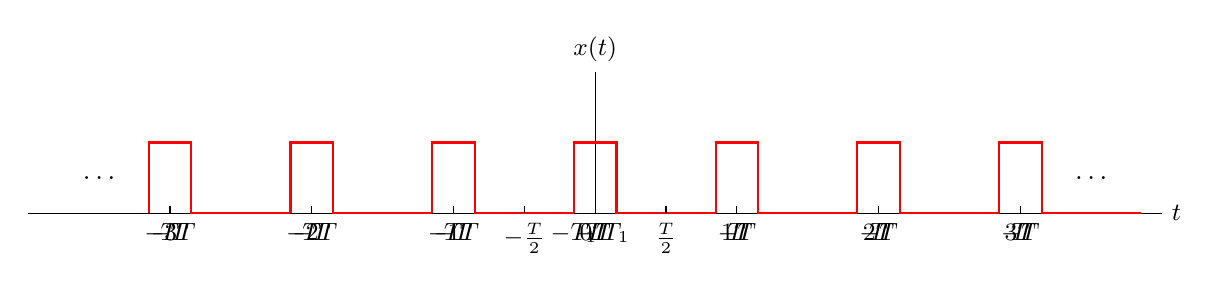
\begin{tikzpicture}[scale=0.9]
	\def\xmin{-7}
	\def\xmax{7}
	\def\ymin{0}
	\def\ymax{2}
	\def\period{2.0}
	\def\T1{0.3}
	\def\A{1}
	
	\edef\pulse{|- ++(2*\T1, \A) |- ++( \period - 2*\T1, -\A)}

	
	\draw (\xmin-1, 0) --(\xmax+1, 0) node[anchor=west] {\small $t$};
	\draw (0, \ymin) --(0, \ymax) node[anchor=south] {\small $x(t)$};
		\foreach \x in {-3, -2, ..., 3}
		{
			\pgfmathmultiply{\period}{\x}
			\edef\position{\pgfmathresult}
			\ifthenelse{\x=0 \OR \x=1 \OR \x=-1}
			{
				%\node at (\position, 0) [anchor=north] {\small $0$};
			}
			{
				
				\node at (\position, 0) [anchor=north] {\small $\x T$};
			}
			\ifthenelse{ \x=1 }
			{
				\node at (\position, 0) [anchor=north] {\small $T$};
			}
			{
			}
			
			\ifthenelse{ \x=-1 }
			{
				\node at (\position, 0) [anchor=north] {\small $-T$};
			}
			{
			}			
			\draw[thick, red] (\position-\T1, 0) \pulse;	
			\draw (\position, 0) -- ++(0,0.1);
			%\pulse{3}{0.4};		
		}
		
		\node at (-\T1, 0) [anchor=north] {\small $-T_1$};
		\node at (\T1, 0) [anchor=north] {\small $T_1$};
		\node at (-\period/2, 0) [anchor=north] {\small $-\frac{T}{2}$};
		\node at (\period/2, 0) [anchor=north] {\small $\frac{T}{2}$};
		\draw (-\period/2, 0) -- ++(0,0.1);
		\draw (\period/2, 0) -- ++(0,0.1);

		\node at (\xmin, \A/2) {$\dots$};
		\node at (\xmax, \A/2) {$\dots$};
\end{tikzpicture}

      \caption{Periodic square wave}\label{fi:example02_periodic_square_wave }
    \end{figure}
\end{frame}

\begin{frame}<beamer>
    \begin{columns}
      \begin{column}{0.5\textwidth}
            \begin{equation*}
                \begin{split}
                   a_0 &= \frac{1}{T} \int_{T}x(t)dt,\\
                   &=  \frac{1}{T} \int_{-T_1}^{T_1}1dt,\\
                   &= \frac{2T_1}{T}.
                \end{split}
            \end{equation*}
            \pause
            \begin{equation*}
                \begin{split}
                   a_k &= \frac{1}{T} \int_{T}x(t)e^{-jk\omega_0 t}dt,\\
                   &=  \frac{1}{T} \int_{-T_1}^{T_1}e^{-jk\omega_0 t},\\
                   &= -\left. \frac{1}{jk\omega_0 T}e^{-jk\omega_0 t}\right|^{T_1}_{-T_1}
                \end{split}
            \end{equation*}
      \end{column}
      \begin{column}{0.5\textwidth}
            \pause
            \begin{equation*}
                \begin{split}
                   a_k &= \frac{2}{k\omega_0 T}\left[\frac{e^{jk\omega_0 t} - e^{-jk\omega_0 t}}{2j}\right]\\
                   a_k &= \frac{2\sin(k\omega_0 T_1)}{k\omega_0 T} = \frac{2\sin(k\omega_0 T_1)}{k\pi}, k \neq 0.
                \end{split}
            \end{equation*}
      \end{column}
    \end{columns}
\end{frame}

\begin{frame}<beamer>
    For $T=4T_1$
    \begin{equation*}
        a_k = 0, \quad k \text{ even}.
    \end{equation*}
    \begin{align*}
        a_1 &= a_{-1} = \frac{1}{\pi}\\
        a_3 &= a_{-3} = \frac{1}{3\pi}\\
        a_5 &= a_{-5} = \frac{1}{5\pi}\\
    \end{align*}
\end{frame} 


\begin{frame}<beamer>[plain,t]
    \begin{figure}
      \centering
      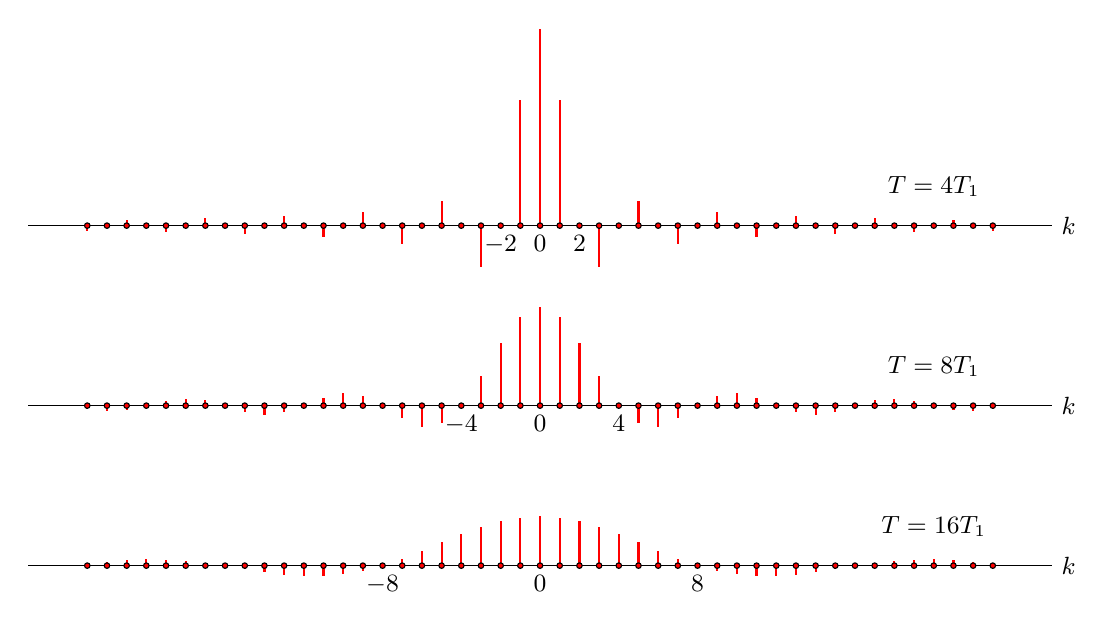
\begin{tikzpicture}[scale=0.5]
	\def\w{{-23,-22,-21,-20,-19,-18,-17,-16,-15,-14,-13,-12,-11,-10,-9,-8,-7,-6,-5,-4,-3,-2,-1,0,1,2,3,4,5,6,7,8,9,10,11,12,13,14,15,16,17,18,19,20,21,22,23}}
	\def\akmag{{-0.013840,0.000000,0.015158,-0.000000,-0.016753,0.000000,0.018724,-0.000000,-0.021221,0.000000,0.024485,-0.000000,-0.028937,0.000000,0.035368,-0.000000,-0.045473,0.000000,0.063662,-0.000000,-0.106103,0.000000,0.318310,0.500000,0.318310,0.000000,-0.106103,-0.000000,0.063662,0.000000,-0.045473,-0.000000,0.035368,0.000000,-0.028937,-0.000000,0.024485,0.000000,-0.021221,-0.000000,0.018724,0.000000,-0.016753,-0.000000,0.015158,0.000000,-0.013840}}


	\begin{scope}	
		\draw (-13, 0) -- (13,0) node[anchor=west] {\small $k$};
		\foreach \k in {-2, 0, 2}
		{
			\node at (\k/2, 0) [anchor=north] {\small $\k$};
		}
		%\node at (0,5) [anchor=south] {\small $Ta_k$};
		
		\foreach \k in {0,1, ..., 46}
		{
			\pgfmathparse{\w[\k]/2}
			\edef\wk{\pgfmathresult}
			\pgfmathparse{\akmag[\k]}
			\edef\akmagk{\pgfmathresult}	
			\draw[thick, red] (\wk, 0) -- ++(0,10*\akmagk);% node [anchor=south] {\small $\akmagk$};
			\ifthenelse{\lengthtest{0 pt = \akmagk pt}}{\draw[fill=red]  (\wk,0) circle (2pt);}{}
		}
			\node at (10, 1) {\small $T= 4T_1$};		
	\end{scope}

%\pause
\def\akmag{{-0.009786,-0.014469,-0.010718,0.000000,0.011846,0.017684,0.013240,-0.000000,-0.015005,-0.022736,-0.017314,0.000000,0.020462,0.031831,0.025009,-0.000000,-0.032154,-0.053052,-0.045016,0.000000,0.075026,0.159155,0.225079,0.250000,0.225079,0.159155,0.075026,0.000000,-0.045016,-0.053052,-0.032154,-0.000000,0.025009,0.031831,0.020462,0.000000,-0.017314,-0.022736,-0.015005,-0.000000,0.013240,0.017684,0.011846,0.000000,-0.010718,-0.014469,-0.009786}}


	\begin{scope}[yshift=-1.8in]
		\draw (-13, 0) -- (13,0) node[anchor=west] {\small $k$};
		\foreach \k in {-4, 0, 4}
		{
			\node at (\k/2, 0) [anchor=north] {\small $\k$};
		}
		%\node at (0,5) [anchor=south] {\small $Ta_k$};
		
		\foreach \k in {0,1, ..., 46}
		{
			\pgfmathparse{\w[\k]/2}
			\edef\wk{\pgfmathresult}
			\pgfmathparse{\akmag[\k]}
			\edef\akmagk{\pgfmathresult}	
			\draw[thick, red] (\wk, 0) -- ++(0,10*\akmagk);% node [anchor=south] {\small $\akmagk$};
			\ifthenelse{\lengthtest{0 pt = \akmagk pt}}{\draw[fill=red]  (\wk,0) circle (2pt);}{}		
		}
			\node at (10, 1) {\small $T= 8T_1$};			
	\end{scope}
%\pause
\def\akmag{{0.005296,0.010231,0.014004,0.015915,0.015478,0.012504,0.007165,-0.000000,-0.008121,-0.016077,-0.022622,-0.026526,-0.026735,-0.022508,-0.013535,0.000000,0.017402,0.037513,0.058816,0.079577,0.098027,0.112540,0.121812,0.125000,0.121812,0.112540,0.098027,0.079577,0.058816,0.037513,0.017402,0.000000,-0.013535,-0.022508,-0.026735,-0.026526,-0.022622,-0.016077,-0.008121,-0.000000,0.007165,0.012504,0.015478,0.015915,0.014004,0.010231,0.005296}}


	\begin{scope}[yshift=-3.4in]
		\draw (-13, 0) -- (13,0) node[anchor=west] {\small $k$};
		\foreach \k in {-8, 0, 8}
		{
			\node at (\k/2, 0) [anchor=north] {\small $\k$};
		}
		%\node at (0,5) [anchor=south] {\small $Ta_k$};
		
		\foreach \k in {0,1, ..., 46}
		{
			\pgfmathparse{\w[\k]/2}
			\edef\wk{\pgfmathresult}
			\pgfmathparse{\akmag[\k]}
			\edef\akmagk{\pgfmathresult}	
			\draw[thick, red] (\wk, 0) -- ++(0,10*\akmagk);% node [anchor=south] {\small $\akmagk$};
			\ifthenelse{\lengthtest{0 pt = \akmagk pt}}{\draw[fill=red]  (\wk,0) circle (2pt);}{}
		}
			\node at (10, 1) {\small $T= 16T_1$};			
	\end{scope}

% 	\begin{scope}[yshift=-1in]
% 		\draw (-4, 0) -- (4,0) node[anchor=west] {\small $k$};
% 		\foreach \k in {0,1, ..., 6}
% 		{			
% 			\pgfmathparse{\w[\k]}
% 			\edef\wk{\pgfmathresult}
% 			\pgfmathparse{\akarg[\k]}
% 			\edef\akargk{\pgfmathresult}	
% 			\pgfmathint{\wk}
% 			\edef\km3int{\pgfmathresult}
% 			\pgfmathsign{\akargk}
%             \def\argsign{\pgfmathresult}		
% 			\ifthenelse{-1=\argsign}{\node at (\wk, 0) [anchor=south] {\small $\km3int$};}{\node at (\wk, 0) [anchor=north] {\small $\km3int$};}
% 			\ifthenelse{-1=\argsign}{\edef\anchor{north}}{\edef\anchor{south}}			
%
% 			\draw[thick] (\wk, 0) -- ++(0,\akargk) node[anchor=\anchor] {\small $\akargk$};;
% 			\ifthenelse{\lengthtest{0 pt = \akargk pt}}{\draw[fill=black]  (\wk,0) circle (2pt);}{}			
% 		}
% 		%\node at (0,1.2) [anchor=south] {\small $\sphericalangle a_k$};				
% 	\end{scope}
\end{tikzpicture} 
      \caption{Plots of scaled Fourier series coefficients $Ta_k$}\label{fi:example02_periodic_square_fs}
    \end{figure}
\end{frame}
